% !TEX root = ../Poissons.tex

\section{Tables}
\label{s:tables}

In this section we present low dimensional computations of the enumeration results obtained above and we connect them to other known combinatorial objects. 

\begin{figure}[h]
\centerline{
\begin{tabular}{r|c}
\textbf{dim} & \textbf{0}  \\
\hline
\textbf{0} & 1  
\end{tabular}
\ \ \
\begin{tabular}{r|cc}
\textbf{dim} & \textbf{0} & \textbf{1}  \\
\hline
\textbf{0} & 3 & 1 \\
\textbf{1} & 1 &  
\end{tabular}
\ \ \
\begin{tabular}{r|ccc}
\textbf{dim} & \textbf{0} & \textbf{1} & \textbf{2}  \\
\hline
\textbf{0} & 17 & 12 & 1 \\
\textbf{1} & 12 &  6 & \\
\textbf{2} & 1 &  & 
\end{tabular}
\ \ \
\begin{tabular}{r|cccc}
\textbf{dim} & \textbf{0} & \textbf{1} & \textbf{2} & \textbf{3} \\
\hline
\textbf{0} & 149 & 162 & 38 & 1 \\
\textbf{1} & 162 & 150 & 24 & \\
\textbf{2} & 38 & 24 & & \\
\textbf{3} & 1 & & &
\end{tabular}
}
\caption{Number of pairs of faces in the cellular image of the diagonal $0$, $1$, $2$ and $3$-dimensional permutahedra.}
\label{t:dim1-3}
\end{figure}

\begin{figure}[h]
\centerline{
\begin{tabular}{r|ccccc}
\textbf{dim} & \textbf{0} & \textbf{1} & \textbf{2} & \textbf{3} & \textbf{4} \\
\hline
\textbf{0} & 1809 & 2660 & 1080 & 110 & 1 \\
\textbf{1} & 2660 & 3540 & 1200 & 80 & \\
\textbf{2} & 1080 & 1200 & 270 & & \\
\textbf{3} & 110 & 80 & && \\
\textbf{4} & 1 & & & &
\end{tabular}
\ \ \
\begin{tabular}{r|cccccc}
\textbf{dim} & \textbf{0} & \textbf{1} & \textbf{2} & \textbf{3} & \textbf{4} & \textbf{5} \\
\hline
\textbf{0} & 28399 & 52635 & 30820 & 6165 & 302 & 1 \\
\textbf{1} & 52635 & 90870 & 67580 & 7785 & 240 & \\
\textbf{2} & 30820 & 47580 & 20480 & 2160 & & \\
\textbf{3} & 6165 & 7785 & 2160 & && \\
\textbf{4} & 302 & 240 & & &&\\
\textbf{5} & 1 & & & &&
\end{tabular}
}
\caption{Number of pairs of faces in the cellular image of the diagonal $4$ and $5$-dimensional permutahedra.}
\label{t:dim4-5}
\end{figure}



\begin{figure}[h]
\centerline{\begin{tabular}{c|c|rrrrrrr|l}
\textbf{Pairs $(F,G) \in \Ima\triangle_{(P,\vec v)}$} & \textbf{Polytopes} & \textbf{0} & \textbf{1} & \textbf{2} & \textbf{3} & \textbf{4} & \textbf{5} & \textbf{6} & \textbf{\cite{OEIS}} \\
\hline
& \text{Associahedra} & 1 & 2 & 6 & 22 & 91 & 408 & 1938 & \OEIS{A000139}  \\
$\dim F + \dim G = \dim P$  & \text{Multiplihedra} & 1 & 2 & 8 & 42 & 254 & 1678 & 11790 &  to appear \\
  & \text{Permutahedra} & 1 & 2 & 8 & 50 & 432 & 4802 & 65536 &  \OEIS{A007334} \\
\hline
  & \text{Associahedra} & 1 & 3 & 13 & 68 & 399 & 2530 & 16965 &  \OEIS{A000260} \\
  $\dim F=\dim G =0$ & \text{Multiplihedra} & 1 & 3 & 17 & 122 & 992 & 8721 & 80920 & to appear \\
  & \text{Permutahedra} & 1 & 3 & 17 & 149 & 1809 & 28399 & 550297 &  \OEIS{A213507} 
\end{tabular}}
\caption{Number of pairs of faces in the cellular image of the diagonal of the associahedra, multiplihedra and permutahedra of dimension $0\leq \dim P \leq 6$, induced by any good orientation vector.}
\label{table:numerology}
\end{figure}


\Guillaume{On garde?}


\subsubsection{Combinatorial formula for facets of the diagonal}

From \cref{thm:facets}, we can deduce a formula for the number of facets of the diagonal:

\begin{proposition}
The number of pairs of ordered partitions of dimension $(k,n-k)$ which correspond to facets of the diagonal is given by: 
\begin{equation}
\frac{1}{k+1}\binom{n+1}{k}(k+1)^{n-k}(n+1-k)^{k}.
\end{equation}
\end{proposition}

\begin{proof}
According to \cref{thm:facets}, pairs of ordered partitions of dimension $(k,n-k)$ which correspond to facets of the diagonal are in one-to-one correspondence with bipartite trees with $k+1$ black vertices, $n-k+1$ white vertices and $n+1$ edges labeled from $1$ to $n+1$.

We do not prove exactly here the proposition but a slightly modified version: 
Rooted bipartite trees with $k+1$ black vertices and $n-k+1$ white vertices such that:
\begin{itemize}
\item a black vertex is distinguished and called \emph{the root}
\item the $n+1$ non-root vertices are labeled,
\item every label between $1$ and $n+1$ is used exactly once.
\end{itemize}
are counted by:
\begin{equation}
\binom{n+1}{k}(k+1)^{n-k}(n+1-k)^{k}.
\end{equation}

Let us construct such a bipartite tree. 

First, there are $\binom{n+1}{k}$ ways to  choose the labels for black vertices (white vertices being labeled by the non-chosen labels). 
We denote by $\mathcal{B}$ this set of labels.

Moreover, the labeled black vertices are different from the root, hence they should have a white parent : there are $n+1-k$ ways to choose the parent of any labeled black vertex. 
We thus have  $(n+1-k)^{k}$ ways to build corollas with labeled black leaves and a white root, called bi-colored corollas (or sometimes just corollas) in the sequel.

Finally, we arrange bi-colored corollas in a rooted bipartite tree by adapting the algorithm which convert a Pr\"ufer code to a tree. 
Here what is called \emph{Pr\"ufer code} is a word of length $n-k$ over the alphabet $\mathcal{B} \cup \{\bullet\}$, where $\bullet$ stands for the non-labeled black vertex. 
Let us start with a word $c=c_1 \ldots c_{n-k} \bullet$ of length $n-k+1$ and the set $\mathcal{T}=\mathcal{S} \cup \{\bullet\}$ of $n-k+2$ bi-colored corollas augmented with the unlabeled black vertex. 
We apply Algorithm \ref{PruferWtoT}. Let us first prove it termination and correctness. The equality 
$\operatorname{length}(c)=\operatorname{Card}(\mathcal{T})-1$ is a loop invariant for the While loop: indeed at each iteration of the loop, the length of $c$ and the number of elements in $\mathcal{T}$ decrease exactly by one. It ensures the termination of the loop and the fact that $\mathcal{T}$ contains a unique element when exiting the loop. Moreover, the set of trees $\mathcal{T}$ contains at each steps exactly one unlabeled black vertex, $k$ labeled black vertices and $n-k+1$ white vertices. Finally, when adding an edge between two trees, one can only get a tree. Moreover, as the edge is added between a white root and the label of a black vertex, the obtained tree is indeed bipartite.

\begin{algorithm}[!ht]
\DontPrintSemicolon
  
  \KwInput{a word $c=c_1 \ldots c_{i}$ and a set $\mathcal{T}$ of $i$ bi-colored trees with white root and one bi-colored tree with an unlabeled black root}
  \KwOutput{a bipartite rooted tree}
  \While{$\operatorname{length}(c)>0$}{
      \tcc{loop invariant: $\operatorname{length}(c)=\operatorname{Card}(\mathcal{T})-1$, at each iteration, the length of $c$ decreases by $1$}
      t $\leftarrow \min\{a \in \mathcal{T} |$ none of the $c_i$ is a label in $a\}$ \tcp*{Here the order is given by the order on the labels of the root (as the tree with a black root does not satisfy the condition)}
      p $\leftarrow$ tree of $\mathcal{T}$ to which belongs the first letter of $c$ \tcp*{Note that it cannot be t itself}
      Remove t and p from $\mathcal{T}$ \tcp*{Decrease the cardinality of $\mathcal{T}$ by two}
      Add an edge between the root of $t$ and the first letter of $c$ and add the obtained tree to $\mathcal{T}$ \tcp*{Increase the cardinality of $\mathcal{T}$ by one}
      Remove the first letter of $c$ \tcp*{Decrease the length of $c$ by one}
  }
  {Return the unique element of $\mathcal{T}$}
  \caption{Pr\"ufer algorithm : from a word to a tree \label{PruferWtoT}}
\end{algorithm}

To prove that this algorithm defines a bijection between the pairs of Pr\"ufer code and set of bipartite rooted trees, let us give the algorithm which convert a rooted bipartite tree in such a pair in Algorithm \ref{PruferTtoW}.


\begin{algorithm}[!ht]
\DontPrintSemicolon
  
  \KwInput{a bipartite rooted tree $A$}
  \KwOutput{a word $c=c_1 \ldots c_{i}$ and a set $\mathcal{T}$ of $i$ bi-colored trees with white root, except one bi-colored tree with an unlabeled black root}
  $c \leftarrow$ empty word \tcp*{}
  $\mathcal{T} \leftarrow$ empty set \tcp*{Initialization}
  \While{$A$ has more than one vertex}{
      \tcc{At each iteration, the number of white vertices decreases by $1$}
      t $\leftarrow \min\{w \in \mathcal{T} | w$ is a white vertex whose children are leaves $\}$ \tcp*{Here the order is the one on white labels}
      $c \leftarrow c$ concatenated with label of the parent of t \tcp*{This label is a black vertex}
      Remove the edge between t and its parent: the root part goes in $A$ and the corolla in $\mathcal{T}$ \tcp*{Increase the cardinality of $\mathcal{T}$ by one}}
  {  Return the pair $(c,\mathcal{T} \cup A)$}
  \caption{Pr\"ufer algorithm : from a tree to a word \label{PruferTtoW}}
\end{algorithm}

This second algorithm terminates as the number of white vertices decreases strictly by one at each iterations. Moreover, every letter added to $c$ is the label of a black vertices, and every tree added to $\mathcal{T}$ is a bi-colored corolla or $\bullet$ (the tree with only the non-labeled black root). Finally, the cardinality of the set of bipartite trees is one more than the length of $c$. As this algorithm is the classical reverse algorithm of the first one, it ends the proof.
\BDO{Do I need to add more details ?}
\end{proof}

\begin{example} Let us apply Pr\"ufer algorithm on an example. Consider the following rooted bipartite tree on the left below, with a red root, and a redrawing of it on the right:
\begin{center}
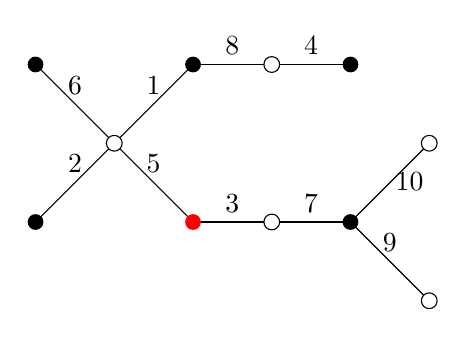
\begin{tikzpicture}
\coordinate (6) at (0,1);
\coordinate (2) at (0,-1);
\coordinate (1) at (2,1);
\coordinate (5) at (1,0);
\coordinate (8) at (3,1);
\coordinate (4) at (4,1);
\coordinate (3) at (3,-1);
\coordinate (7) at (4,-1);
\coordinate (9) at (5,-2);
\coordinate (10) at (5,0);
\coordinate (r) at (2,-1);
\draw (6)--(5) node[midway, above]{6};
\draw (2)--(5) node[midway, above]{2};
\draw (1)--(5) node[midway, above]{1};
\draw (r)--(5) node[midway, above]{5};
\draw (r)--(3) node[midway, above]{3};
\draw (3)--(7) node[midway, above]{7};
\draw (7)--(9) node[midway, above]{9};
\draw (7)--(10) node[near end, below]{10};
\draw (1)--(8) node[midway, above]{8};
\draw (8)--(4) node[midway, above]{4};
\fill (6) circle(0.1);
\fill (2) circle(0.1);
\fill (1) circle(0.1);
\fill[red] (r) circle(0.1);
\fill (4) circle(0.1);
\fill (7) circle(0.1);
\fill[draw,fill=white] (5) circle(0.1);
\fill[draw,fill=white] (3) circle(0.1);
\fill[draw,fill=white] (8) circle(0.1);
\fill[draw,fill=white] (9) circle(0.1);
\fill[draw,fill=white] (10) circle(0.1);
\end{tikzpicture}
\hspace{1cm}
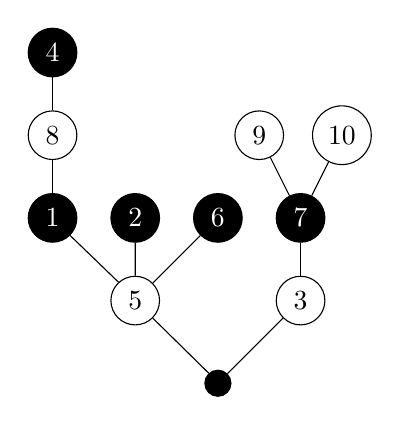
\begin{tikzpicture}[grow=up, scale=0.7,  level 1/.style={sibling distance=3cm},
    level 2/.style={sibling distance=1.5cm}]
\node[draw, circle, fill=black]{}
   child{node[draw, circle]{3}
      child{node[draw, circle, fill=black, text=white]{7}
         child{node[draw, circle]{10}
         }
         child{node[draw, circle]{9}}
      }   
   }
   child{node[draw, circle]{5}
      child{node[draw, circle, fill=black, text=white]{6}
      }   
      child{node[draw, circle, fill=black, text=white]{2}
      }   
      child{node[draw, circle, fill=black, text=white]{1}
         child{node[draw, circle]{8}
            child{node[draw, circle, fill=black, text=white]{4}}         
         }
      }   
   };
\end{tikzpicture}
\end{center}
Separating corollas with a Pr\"ufer algorithm, we get the word $1 \bullet 7 7$ and the following set of corollas:
\begin{equation*}
\left \lbrace 
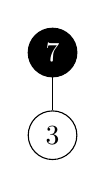
\begin{tikzpicture}[grow=up, scale=0.7, baseline=10]
\node[draw, circle]{3}
      child{node[draw, circle, fill=black, text=white]{7}};
 \end{tikzpicture},
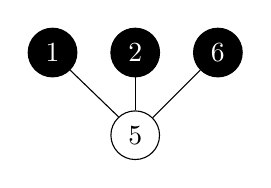
\begin{tikzpicture}[grow=up, scale=0.7, baseline=10]
\node[draw, circle]{5}
      child{node[draw, circle, fill=black, text=white]{6}
      }   
      child{node[draw, circle, fill=black, text=white]{2}
      }   
      child{node[draw, circle, fill=black, text=white]{1}
      }   ;
 \end{tikzpicture}, 
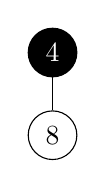
\begin{tikzpicture}[grow=up, scale=0.7, baseline=10]
\node[draw, circle]{8}
            child{node[draw, circle, fill=black, text=white]{4}} ;
 \end{tikzpicture},
 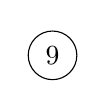
\begin{tikzpicture}[grow=up, scale=0.7, baseline=10]
\node[draw, circle]{9};
 \end{tikzpicture},
  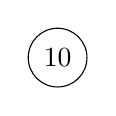
\begin{tikzpicture}[grow=up, scale=0.7, baseline=10]
\node[draw, circle]{10};
 \end{tikzpicture}
  \right \rbrace
\end{equation*}
This set of corollas can be viewed as a function $f$ from the set of labelled black vertices $\{1,2,4,6,7\}$ to the set of white vertices $\{3,5,8,9,10\}$ satisfying $f(1)=f(2)=f(6)=5$, $f(7)=3$ and $f(4)=8$.
\end{example}
